%%%%%%%%%%%%%%%%%%%%%%%%%%%%%%%%%%%%%%%%%%%%%%%%%%%%%%%%%%%%%%%%%%%%%%%%%%%%%%%
%Objetivo: Realizar um estudo de modo a entender as funcionalidades oferecidas
%por uma FGRM de modo à caracterizá-las e classificá-las
%Autor: Vagner Clementino <vagnercs@dcc.ufmg.br>
% 		Rodolfo Resende	<rodolfo@dcc.ufmg.br>
%Criação: qua set 28 11:25:03 BRT 2016
%Modificação: qui mar  9 20:53:27 BRT 2017
%Revisão: dom fev 26 20:24:14 BRT 2017
%%%%%%%%%%%%%%%%%%%%%%%%%%%%%%%%%%%%%%%%%%%%%%%%%%%%%%%%%%%%%%%%%%%%%%%%%%%%%%%
\chapter{Um Estudo sobre as Funcionalidades das FGRMs}
\label{ch:caracterizacao_ferramentas}

\section{Introdução}
\label{sec:caracterizacao_intro}
Quando uma empresa ou um projeto de software de código aberto decide adotar uma
Ferramenta de Gerenciamento de Requisições de Mudança~-~FGRM um possível desafio
é encontrar aquela que melhor atenda suas necessidades. Um possível fundamento
de seleção é o conjunto de funcionalidades oferecidas pelo software. Outros
critérios podem envolver o custo e o suporte pós-venda da ferramenta. De maneira
relacionada, o pesquisador que estuda propostas de melhorias para as FGRMs pode
estar interessado em analisar o conjunto de funções que permita caracterizar
este tipo de software.

O número de FGRMs disponíveis quando esta dissertação foi escrita era bastante
elevado. Em uma inspeção inicial, verificamos a existência de mais de
\textit{50} ferramentas fornecidas comercialmente ou em código
aberto\footnote{\url{https://en.wikipedia.org/wiki/Comparison_of_issue-tracking_systems}}.
Apesar das diversas opções disponíveis, ao bem do nosso conhecimento,
desconhecemos estudos que avaliem sistematicamente as funcionalidades oferecidas
por este tipo de ferramenta. Entendemos que a partir de um conjunto
compartilhado de funções/comportamento seja possível caracterizar as FGRMs, ao
mesmo tempo que possibilita avaliar a contribuição de novas funcionalidades
propostas na li\-te\-ra\-tu\-ra, conforme discutido no
Capítulo~\ref{ch:mapeamento-sistematico}. Para alcançarmos este objetivo,
realizamos um estudo exploratório visando coletar as funcionalidades presentes
nas FGRMs. Um estudo exploratório está preocupado com a análise do objeto em
sua configuração natural e deixando que as descobertas surjam da própria
observação~\cite{wohlin2012experimentation}. Neste tipo de estudo nenhuma
hipótese é previamente definida.

O trabalho descrito neste capítulo consistiu na leitura da documentação
disponível na Internet de algumas FGRMs de modo a sistematizar as
funcionalidades o\-fe\-re\-ci\-das por cada ferramenta. As funções foram
coletadas e organizadas utilizando a técnica de Cartões de Classificação
(Sorting Cards)~\cite{5070993, rugg2005sorting}. Devido ao alto volume de
ferramentas disponíveis e ao esforço necessário para analisar a documentação de
todas elas, optamos por realizar este estudo com um conjunto de 6 ferramentas
que foram escolhidas com a ajuda de profissionais envolvidos em manutenção de
software. Através de um levantamento por meio de questionário (survey) onde os
profissionais definiram quais FGRM eram as mais representativas dentre uma lista
previamente definida. A representatividade neste contexto não está no número de
projetos que utiliza determinada ferramenta, mas pelas caraterísticas que o
software possui e que o torna diferenciável dentro do seu domínio.

\todobegin{Revisar este parágrafo para adequar a nova estrutura do capítulo}
Este capítulo está organizado da seguinte forma: na
Seção~\ref{sec:objetivo_do_capítulo} discutimos os objetos deste capítulo; na
Seção~\ref{sec:metodologia} apresentamos o método utilizado na condução do
estudo, em especial a técnica de Cartões de Ordenação e o levantamento realizado
com os profissionais para escolher as ferramenta do estudo.
\todoend

\section{Objetivo do Capítulo}
\label{sec:caracterizacao_objetivo_do_capítulo}

O objetivo inicial deste capítulo é apresentar e discutir as principais
funcionalidades das FGRMs que dão suporte ao desenvolvimento e manutenção de
software. Tomando como ponto de partida um conjunto de sistemas definidos como
os mais relevantes escolhidos por meio de um levantamento(survey) com o uso de
questionário. Em um segundo momento, o foco foi caracterizar este tipo de
ferramenta tomando como base as funcionalidades oferecidas pelos softwares.
Conforme já exposto, a literatura em Manutenção de Software apresenta diferentes
nomenclaturas para este tipo de ferramenta (Sistema de Controle de Defeito~-~Bug
Tracking Systems, Sistema de Gerenciamento da Requisição~-~Request Management
System, Sistemas de Controle de Demandas (SCD)~-~Issue Tracking Systems), sem,
contudo, se preocupar em diferenciá-las.

Acreditamos que o resultado deste estudo permitirá compreender melhor este tipo
de software tomando como base o conjunto de funções que eles oferecem aos seus
usuários. Também será possível propor novas funcionalidades ou melhorias das
existentes tendo em vista a possibilidade de determinar o conjunto mínimo de
comportamentos deste tipo de ferramenta.

\section{Metodologia}
\label{sec:metodologia}

A fim de determinarmos o conjunto de funcionalidades das FGRMs realizamos um
estudo exploratório dividido em três etapas que estão listadas a seguir. O
resultado obtido em etapa foi utilizado para subsidiar as atividades do etapa
subsequente. O início de uma nova fase do trabalho era precedido de uma
avaliação geral com o objetivo de verificar possíveis inconsistências e
avaliação das lições aprendidas.

\begin{enumerate}[(i)]
	\item Seleção das Ferramentas
	\item Inspeção da Documentação
	\item Agrupamento das Funcionalidades
\end{enumerate}

\subsection{Seleção das Ferramentas}
\label{subsec:selecao-ferramentas}

A primeira etapa consistiu da definição das ferramentas que seriam utilizadas no
estudo. A partir de uma pesquisa na Internet obtivemos um conjunto inicial de 50
ferramentas\footnote{\url{https://en.wikipedia.org/wiki/Comparison_of_issue-tracking_systems}}
que podem ser visualizadas no Apêndice~\ref{ch:app-lista-fgrm}. Devido ao esforço
necessário e a dificuldade de realizar a análise em cada uma daquelas
ferramentas, optamos por escolher um subconjunto de sistemas que fossem mais
representativos, tomando como base a opinião de profissionais envolvidos em
manutenção e desenvolvimento de software. A representatividade neste caso
corresponde a opinião do profissional sobre notoriedade que a ferramenta possui
dentro do seu domínio de aplicação em comparação com as demais que lhe foram
apresentadas ou outras do qual o profissional tenha prévio conhecimento.

\subsubsection{Desenho da Pesquisa com Profissionais}
\label{ssub:metodologia_desenho_da_pesquisa_com_profissionais}

A opinião dos profissionais foi obtida mediante a realização de uma pesquisa de
opinião (survey~\cite{wohlin2012experimentation}) realizada com o uso de um
formulário eletrônico. O formulário foi estruturado em duas partes principais: a
formação de base do participante (background) e a avaliação das ferramentas. Na
primeira parte estávamos interessados em conhecer as características do
respondente. Esta informação é relevante tendo em vista que, como descreveremos
a seguir, o questionário foi replicado em três grupos distintos de
profissionais. Na segunda parte apresentamos as ferramentas e foi solicitado aos
participantes que avaliassem a relevância de cada uma delas através de questões
de múltipla escolha. As opções de respostas foram estruturadas em escala do tipo
Likert~\cite{robbins2011plotting}. Também foi disponibilizado aos participantes
um campo de texto livro no qual era possível informar FGRMs que ele entenda por
relevante, mas que não estava na lista que lhe foi apresentada. Para estas
ferramentas que foram citadas de forma espontânea foi atribuído um grau de
importância igual ``Muito relevante'' conforme Tabela~\ref{tab:graus_relevancia}
no cálculo da métrica de relevância conforme
equação~\ref{eq:escolha_ferramenta}.

Antes da efetiva aplicação do questionário em alguma amostra da população do
estudo, o documento foi validado em um processo de três etapas. Na primeira
parte foi solicitado a dois pesquisadores experientes da área de Engenharia de
Software que avaliassem o formulário. A partir das sugestões obtidas dos
pesquisadores foram realizadas adequações no documento. Após as alterações uma
nova versão do formulário foi enviada para dois profissionais envolvidos
diretamente em manutenção de software. O critério utilizado para seleção dos
profissionais foi o tempo de experiência com desenvolvimento e manutenção de
software, que era em média de 10 anos. O formulário foi modificado com as
sugestões dos profissionais e isso finaliza a segunda etapa de validação. A
última etapa consistiu na realização de um piloto com dez profissionais que
trabalham em um setor de uma empresa pública de informática. Os profissionais
tiveram que preencher o questionário, contudo, foram adicionadas questões
adicionais onde era possível inserir sugestões de melhoria. O resultado deste
processo de validação é o questionário presente no
Apêndice~\ref{ch:app-form-selecao-ferramentas}. Como o público-alvo do questionário
poderia incluir desenvolvedores de diferentes nacionalidades foi construído uma
versão em língua inglesa do formulário.

A população de interesse deste levantamento é o conjunto de profissionais
envolvidos em manutenção de software. Naturalmente é difícil definir o tamanho e
características desta população de modo a mensurar uma amostra significativa.
Neste sentido, visando minimizar enviesamento deste estudo, o questionário
foi replicado em três grupos:

\begin{description}
	\item[Grupo 01:] Profissionais de empresa pública e privada de
			desenvolvimento e manutenção de software.
	\item[Grupo 02:] Profissionais que contribuem em projetos de
		código aberto
	\item[Grupo 03:] Profissionais que participam de grupos de
		interesse sobre desenvolvimento e manutenção de software em uma rede
		social profissional (LinkedIn) ou aqueles que participam de discussão
		sobre este assunto em uma rede social (Stack Overflow).
\end{description}

Os participantes que compõem cada grupo foram escolhidos conforme critérios que
são detalhados no Capítulo~\ref{ch:pesquisa-profissionais}. A reutilização desta
base de desenvolvedores se deu por conta de ambos os estudos compartilharem a
mesma população de interesse, podendo neste caso compartilhar a mesma amostra.

\subsubsection{Critérios de Seleção}
\label{ssub:metodologia_criterios_selecao}

Com base nos dados obtidos da pesquisa com os profissionais, as FGRMs foram
classificadas como \textit{''ferramentas''} e \textit{''serviços da internet''}
utilizando a documentação do software. O primeiro grupo representa os softwares
que são capazes de serem implantados na infraestrutura do seu cliente e permite
algum grau de personalização de pelo menos um dos componentes, como por exemplo,
o banco de dados utilizado. No segundo grupo estão os software que ofertam a
gerência das RMs mediante uma arquitetura do tipo Software como Serviço
(Software as Service)~\cite{fox2013engineering}, onde certos tipos de alterações
no comportamento do software são mais restritas. Acreditamos que ao escolher
ferramentas dos dois tipos iremos cobrir uma grande parte do domínio de
aplicação das FGRMs. Optamos por escolher~\textit{06 ferramentas} para o
estudo, sendo três de cada um dos grupos.

Para seleção das ferramentas utilizados a formula apresentada na
Equação~\ref{eq:escolha_ferramenta}.  Atribuímos a métrica $r_i$ que representa
a relevância de determinada ferramenta $f_i$. A métrica é calculada somando a
frequência de cada um dos graus de relevância apresentado na
Tabela~\ref{tab:graus_relevancia} multiplicado pela pelo grau de relevância
descrito na mesma tabela.

\begin{equation}
\label{eq:escolha_ferramenta}
r_i = \sum_{i=1}^{n} f_i \times w_j
\end{equation}

A documentação de algumas ferramentas, em especial aquelas que adotam uma
arquitetura cliente/servidor e necessitam de um certo grau de administração,
dividem as funcionalidades do software entre aquelas com foco no usuário final e
ad\-mi\-nis\-tra\-do\-res. Nestes casos, optamos por coletar as funcionalidades
cujo o foco seja o usuário da FGRM, tendo em vista que administradores deste
tipo de software não estarem entre no público-alvo desta dissertação.

\begin{table}[htb]
\centering
	\resizebox{0.6\linewidth}{!}{%
\begin{tabular}{|clc|}
\hline
\textbf{$j$} & \textbf{Grau de Relevância} & \textbf{Peso($w_j$)} \\ \hline
1 & Não conheço a ferramenta & 1 \\
2 & Nada relevante & 2 \\
3 & Pouco relevante & 3 \\
4 & Pouco relevante & 4 \\
5 & Muito relevante & 5 \\ \hline
\end{tabular}%
}
\caption{Graus de Relevância}
\label{tab:graus_relevancia}
\end{table}

\subsection{Inspeção da Documentação}
\label{subsec:inspecao_doumentacao}

Nesta etapa do trabalho realizamos a leitura do material disponível na Internet
para cada uma das ferramentas que foram selecionadas conforme critérios
descritos na Subseção~\ref{ssub:metodologia_criterios_selecao}. Entre estes
materiais utilizamos manuais do usuário e do desenvolvedor e notas de
lançamento. Para cada uma das FGRMs optamos por estudar a última versão estável
do software a fim de analisarmos o que há de mais novo disponível aos usuários.
A Tabela~\ref{tab:fgrm-docs} apresenta as ferramentas analisadas e o elo de
ligação para cada documentação utilizada nesta dissertação. Para aquelas ferramentas
que apresentam documentação em mais de um i\-di\-o\-ma optamos por utilizar
aquela escrita em inglês por entendermos ser a que esteja mais atualizada.

\begin{table}[htpb]
\centering
\resizebox{\textwidth}{!}{%
\begin{tabular}{|l|l|}
\hline
\multicolumn{1}{|c|}{\textbf{Nome da Ferramenta}} & \multicolumn{1}{c|}{\textbf{Elo de Ligação}} \\ \hline
Bugzilla & \url{https://www.bugzilla.org/features/} \\
Github Issue Tracking System & \url{https://github.com/blog/411-github-issue-tracker} \\
Github Issue Tracking System & \url{https://github.com/features} \\
Github Issue Tracking System & \url{https://guides.github.com/features/issues/} \\
Gitlab Issue Tracking System & \url{http://docs.gitlab.com/ce/user/project/labels.html} \\
Gitlab Issue Tracking System & \url{https://about.gitlab.com/2016/08/22/announcing-the-gitlab-issue-board/} \\
Gitlab Issue Tracking System & \url{https://about.gitlab.com/solutions/issueboard/} \\
Gitlab Issue Tracking System & \url{https://docs.gitlab.com/ee/user/project/description\_templates.html} \\
Gitlab Issue Tracking System & \url{https://docs.gitlab.com/ee/user/project/issues/automatic\_issue\_closing.html} \\
Gitlab Issue Tracking System & \url{https://docs.gitlab.com/ee/workflow/issue\_weight.html} \\
Gitlab Issue Tracking System & \url{https://docs.gitlab.com/ee/workflow/milestones.html} \\
Gitlab Issue Tracking System & \url{https://docs.gitlab.com/ee/workflow/time\_tracking.html} \\
JIRA & \url{https://br.atlassian.com/software/jira/features} \\
MantisBT & \url{https://www.mantisbt.org/wiki/doku.php/mantisbt:features} \\
Redmine & \url{http://www.redmine.org/projects/redmine/wiki/Features} \\ \hline
\end{tabular}%
}
\caption{Documentações utilizadas no processo de coleta de dados.}
\label{tab:fgrm-docs}
\end{table}

Os dados obtidos da leitura do material disponíveis para cada ferramenta foram
sistematizados por meio de técnica denominada \textit{Cartões de
	Classificação~-~Sorting Cards}. Cartões de Classificação é um técnica de
elicitação de conhecimento, de baixo custo e com foco no usuário, largamente
utilizada em arquitetura informacional para criar modelos mentais e derivar
taxonomias da entrada utilizada~\cite{just2008towards}. Ela envolve a
categorização de um conjunto de cartões em grupos distintos de acordo com algum
critério previamente definido~\cite{mcgee2009software}. O estudo de Maiden e
outros~\cite{maiden1996acre} sugere que a técnica de Cartões de Classificação é
uma das mais úteis para aquisição de conhecimento de dados, em contraste ao
conhecimento de comportamento ou de processo.

Existem três principais fases dentro do processo de classificação dos cartões:
($i$) preparação, no qual participantes ou o conteúdo dos cartões são selecionados;
($ii$) execução, onde o cartões são organizados em grupo significativos com um
título que o descreve; e por fim, ($iii$) análise, no qual os cartões são
sistematizados para formar hierarquias mais abstratas que são usadas para
deduzir resultados. No processo tradicional de Cartões Ordenados cada declaração
realizada por um participante resulta na criação de exatamente um único
cartão~\cite{just2008towards}. Contudo, no nosso caso, foi realizada a divisão
da documentação da ferramenta por cada funcionalidade encontrada. Neste sentido,
cada funcionalidade obtida mediante a inspeção da documentação foi mapeada em
único cartão.

Os cartões foram organizados de modo que continham o nome e a versão da
ferramenta analisada; a URL da documentação utilizada; o nome da funcionalidade
coletada, que consiste de uma descrição breve conforme existente na
documentação; descrição detalhada da funcionalidade, cujo objetivo é facilitar o
processo de agrupamento que será descrito na próxima seção. O
Apêndice~\ref{ch:app-form-cartoes-ordenados} apresenta um formulário que representa
os cartões utilizados nesta dissertação. Nas Figura~\ref{fig:documentacao_bugzilla}
e~\ref{fig:exemplo_cartao_ordenado} é possível visualizar, respectivamente, a
documentação de uma funcionalidade da FGRM Bugzilla e o cartão que foi gerado
para a mesma.

\todobegin{Incluída figuras para incluir a coleta dos dados da documentação das
ferramentas}
\begin{figure}[htpb]
	\centering
	\includegraphics[width=0.8\linewidth]{./chapter-estudo-funcionalidades-fgrm/img/documentacao_bugzilla.png}
	\caption{Exemplo de documentação de uma funcionalidade da FGRM Bugzilla}
	\label{fig:documentacao_bugzilla}
\end{figure}

\begin{figure}[htpb]
	\centering
	\includegraphics[width=0.8\linewidth]{./chapter-estudo-funcionalidades-fgrm/img/exemplo_cartao_ordenado.png}
	\caption{Exemplo de um cartão ordenado para uma funcionalidade da FGRM
		Bugzilla}
	\label{fig:exemplo_cartao_ordenado}
\end{figure}
\todoend

\subsection{Agrupamento das Funcionalidades}
\label{subsec:agrupamento_fucionalidades}

Esta etapa tem por objetivo agrupar as funcionalidades que aparecem com
nomenclatura distintas em diferentes ferramentas, mas que apresentam o mesmo
significado. Cabe ressaltar que o agrupamento de algumas funcionalidades pode
depender de uma análise subjetiva do responsável pela atividade. Neste sentido,
a fim de evitar algum tipo de viés o agrupamento foi realizado em duas etapas:

\begin{description}
	\item[Análise Individual] Neste etapa o autor e um outro especialista
		realizam de forma separada os agrupamentos que acharem necessários.
	\item[Anaĺise Compartilhada] Em um segundo momento tanto o autor quanto o
		es\-pe\-ci\-a\-lis\-ta discutem as possíveis divergências até que um
		consenso seja obtido.
\end{description}

Após o processo de agrupamento foi possível realizar a categorização das
funcionalidades das ferramentas. Os resultados do processo de agrupamento são
apresentados e discutidos nas próximas seções.

\section{Resultados}
\label{sec:resultados}

Nesta seção iniciaremos apresentando o resultado do processo de escolha das
ferramentas que foi realizado mediante um levantamento com questionário.
Começamos por apresentar o perfil dos participantes e em seguida exibimos as
categorias resultantes do processo de ordenamento dos cartões.

\subsubsection{Perfil dos Participantes}
\label{ssub:Perfil dos Participantes}
Ao final do levantamento realizado com profissionais obtivemos um total de
\textit{52} respostas. Os profissionais que participaram são em sua maioria
desenvolvedores conforme pode ser verificado na
Figura~\ref{fig:grafico_escolha_ferramentas_funcao_participantes}.

\begin{figure}[htpb]
	\centering
	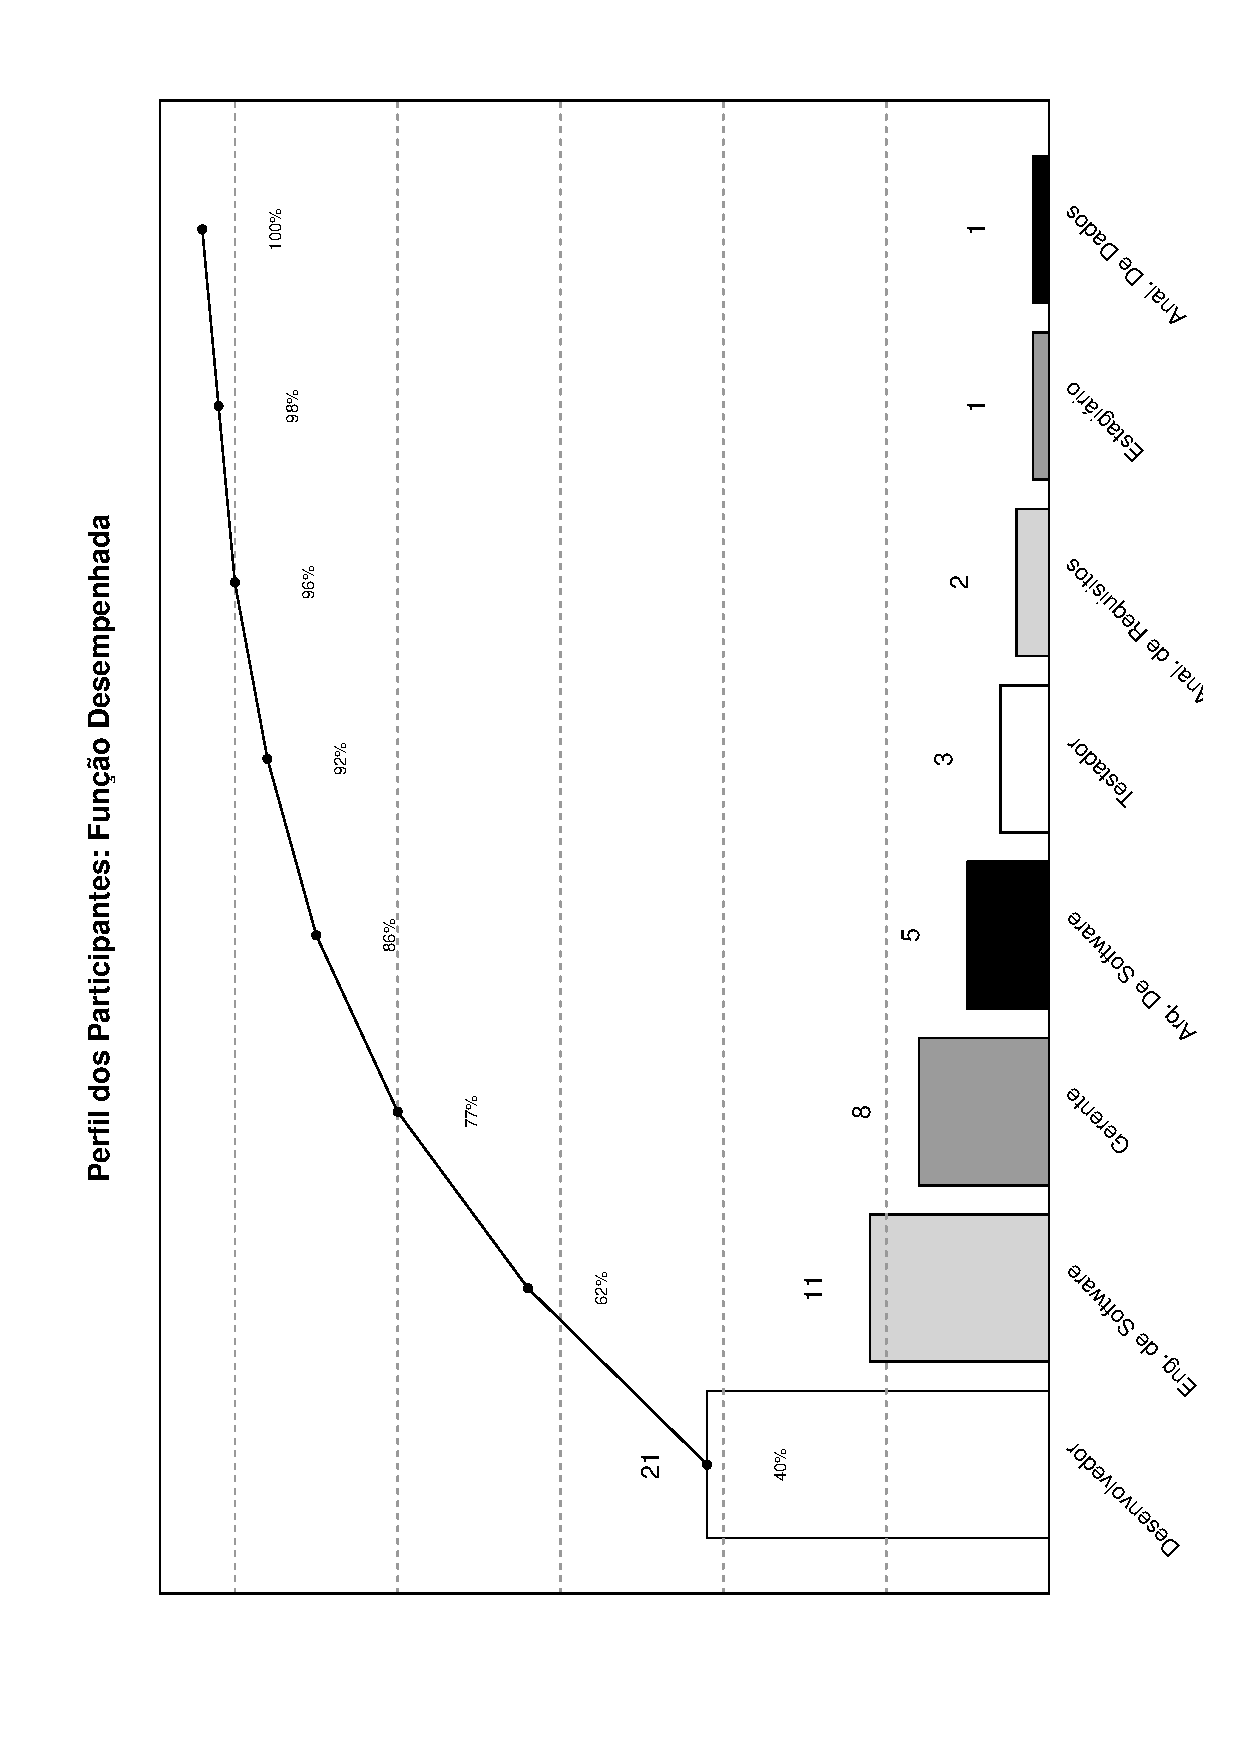
\includegraphics[width=0.8\linewidth]{./chapter-estudo-funcionalidades-fgrm/img/grafico_escolha_ferramentas_funcao_participantes.pdf}
	\caption{Funções desempenhadas pelos participantes}
	\label{fig:grafico_escolha_ferramentas_funcao_participantes}
\end{figure}

O grupo de respondentes também incluem Engenheiros de Software, Gerentes de
Equipe e Arquitetos de Software que, junto com os Desenvolvedores, representam
mais de 80\% do total. Com relação a experiência verificamos que a maior parte
possui entre 3 e 10 anos, conforme pode ser verificado pela
Figura~\ref{fig:grafico_escolha_ferramentas_tempo_experiencia}.

\begin{figure}[htpb]
	\centering
	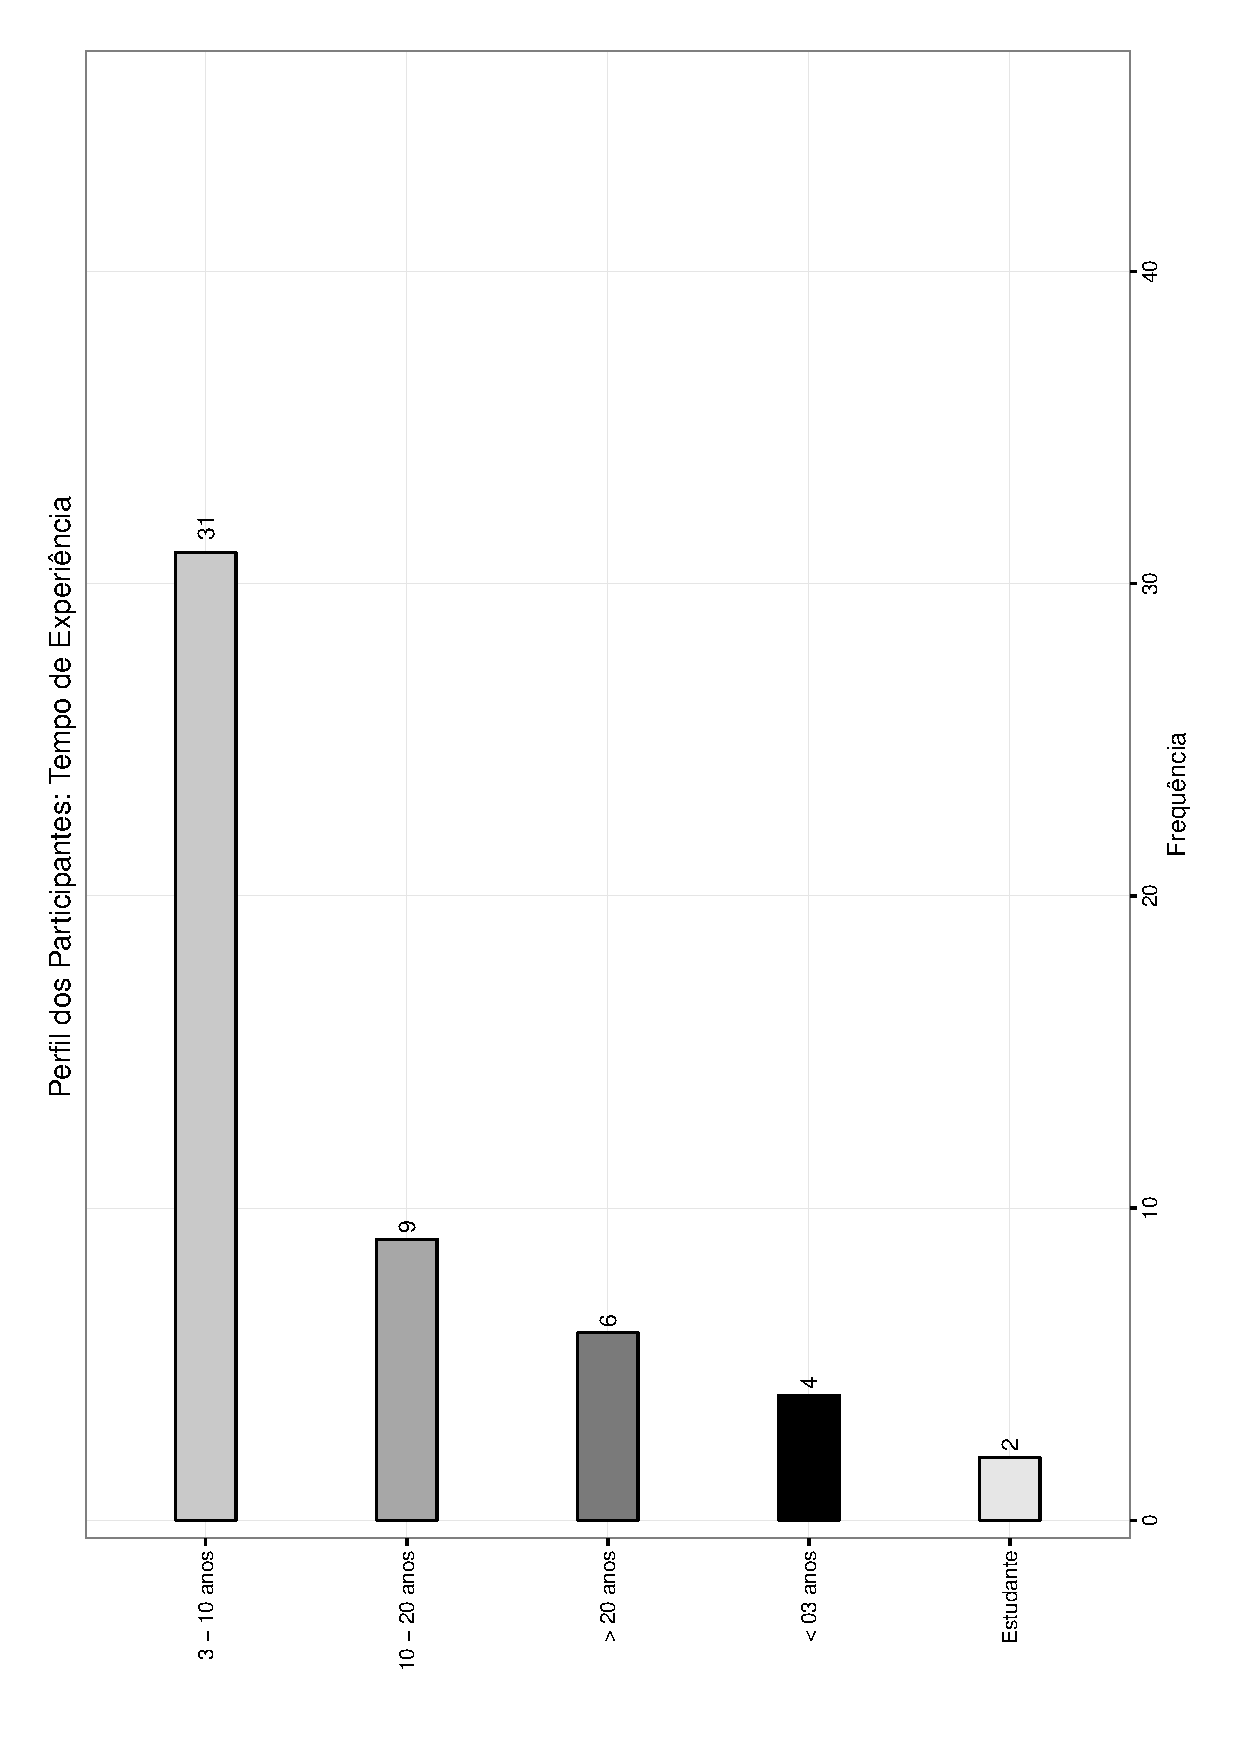
\includegraphics[width=0.8\linewidth]{./chapter-estudo-funcionalidades-fgrm/img/grafico_escolha_ferramentas_tempo_experiencia.pdf}
	\caption{Tempo de Experiência}
	\label{fig:grafico_escolha_ferramentas_tempo_experiencia}
\end{figure}

Com relação ao tamanho da equipe em que os participantes fazem parte,
verificamos uma prevalência de equipes de médio ( mais do que 10 membro) e
pequenas (2 a 5 membros) porte. A
Figura~\ref{fig:grafico_escolha_ferramentas_tamanho_equipe} exibe o tamanho da
equipe dos participantes. Por sua vez, estas equipes estão predominantemente em
empresas privadas de software. Com relação ao local de trabalho verificamos
ainda que o segundo posto em número par\-ti\-ci\-pan\-tes ficou para empresas
que pertencem ao setor governamental. Esta distribuição pode ser visualizada na
Figura~\ref{fig:grafico_escolha_ferramentas_local_trabalho}.

\begin{figure}[htpb]
	\centering
	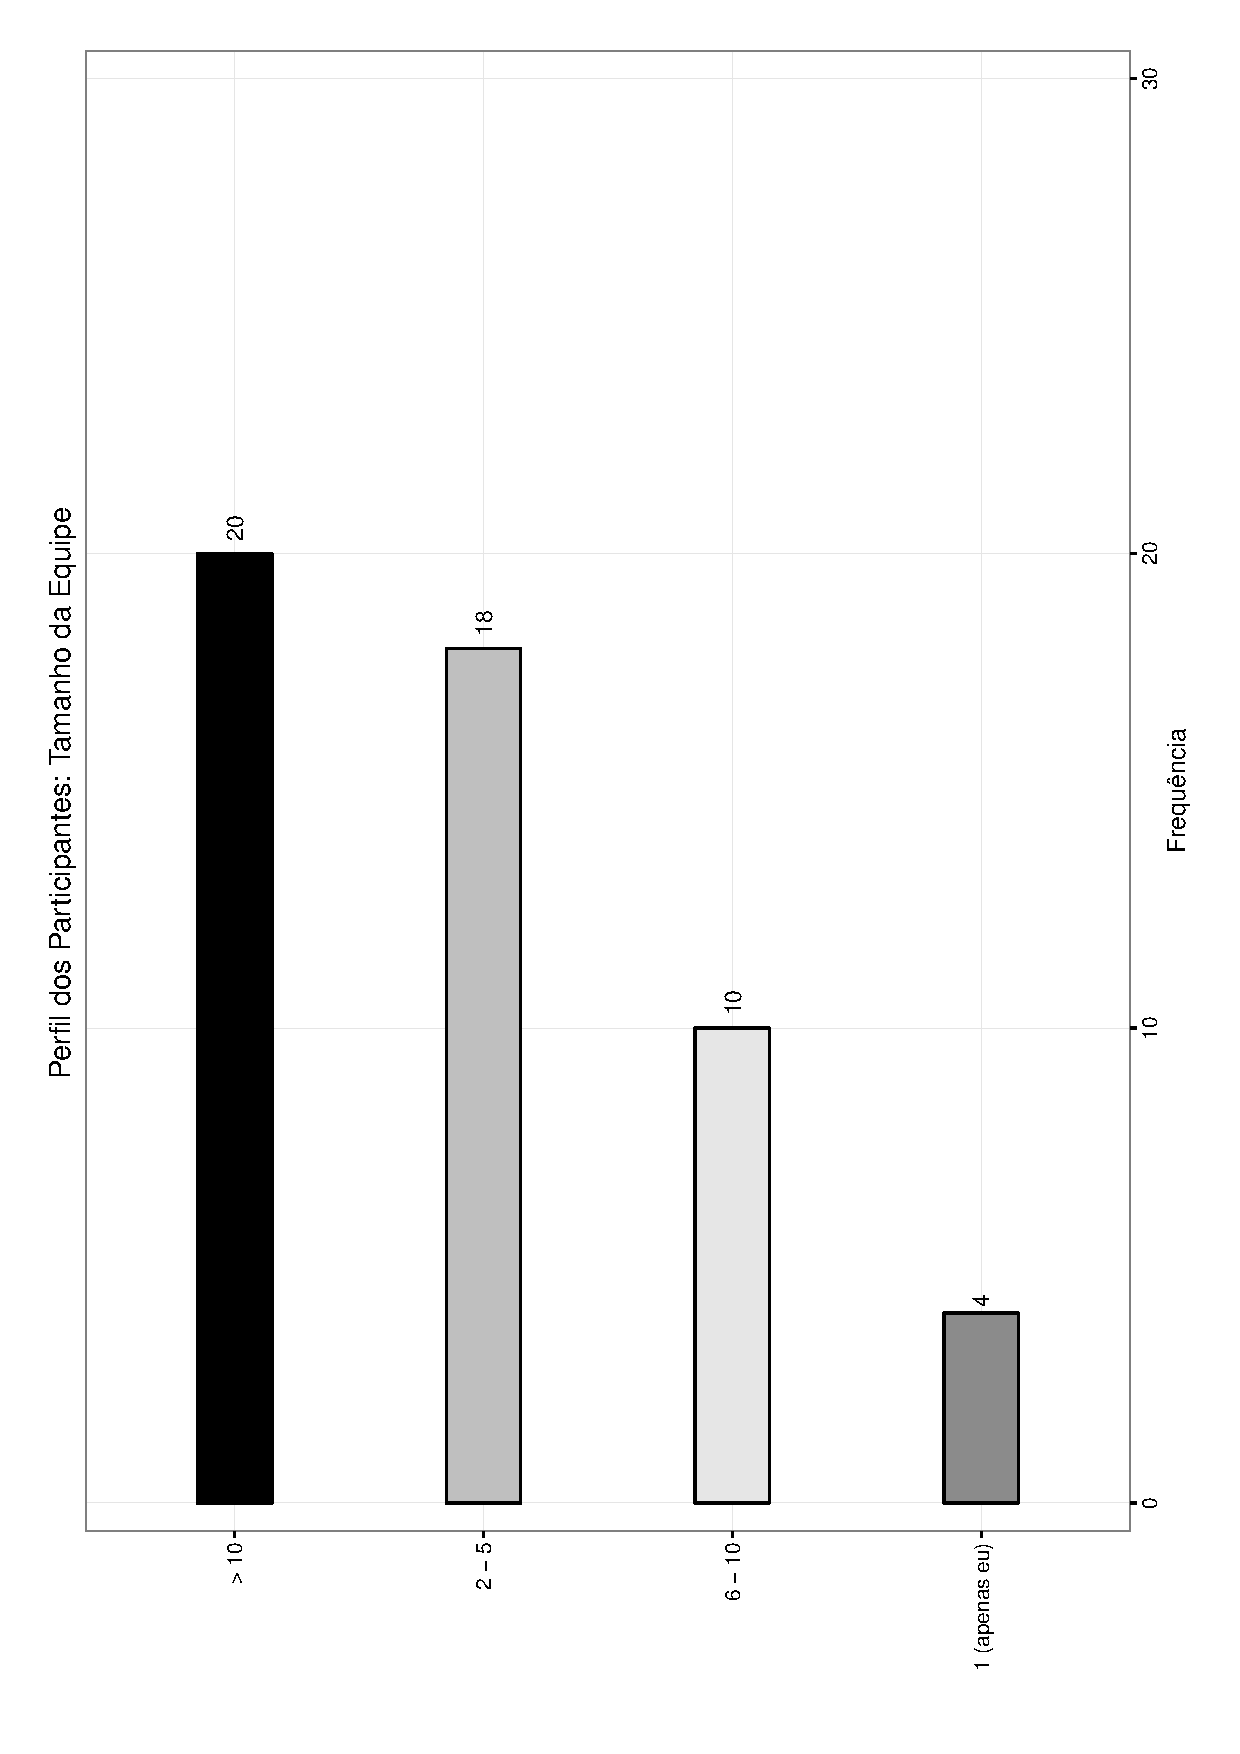
\includegraphics[width=0.8\linewidth]{./chapter-estudo-funcionalidades-fgrm/img/grafico_escolha_ferramentas_tamanho_equipe.pdf}
	\caption{Tamanho da Equipe}
	\label{fig:grafico_escolha_ferramentas_tamanho_equipe}
\end{figure}

Em geral, podemo caracterizar o participante típico como um desenvolvedor entre
três e dez anos de experiência trabalhando em uma empresa privada de
desenvolvimento de software que com uma equipe de aproximadamente dez membros.
Segundo o nosso entendimento, como este perfil um profissional tem o
conhecimento necessário para nos ajudar no processo de escolha das ferramentas.

\begin{figure}[htpb]
	\centering
	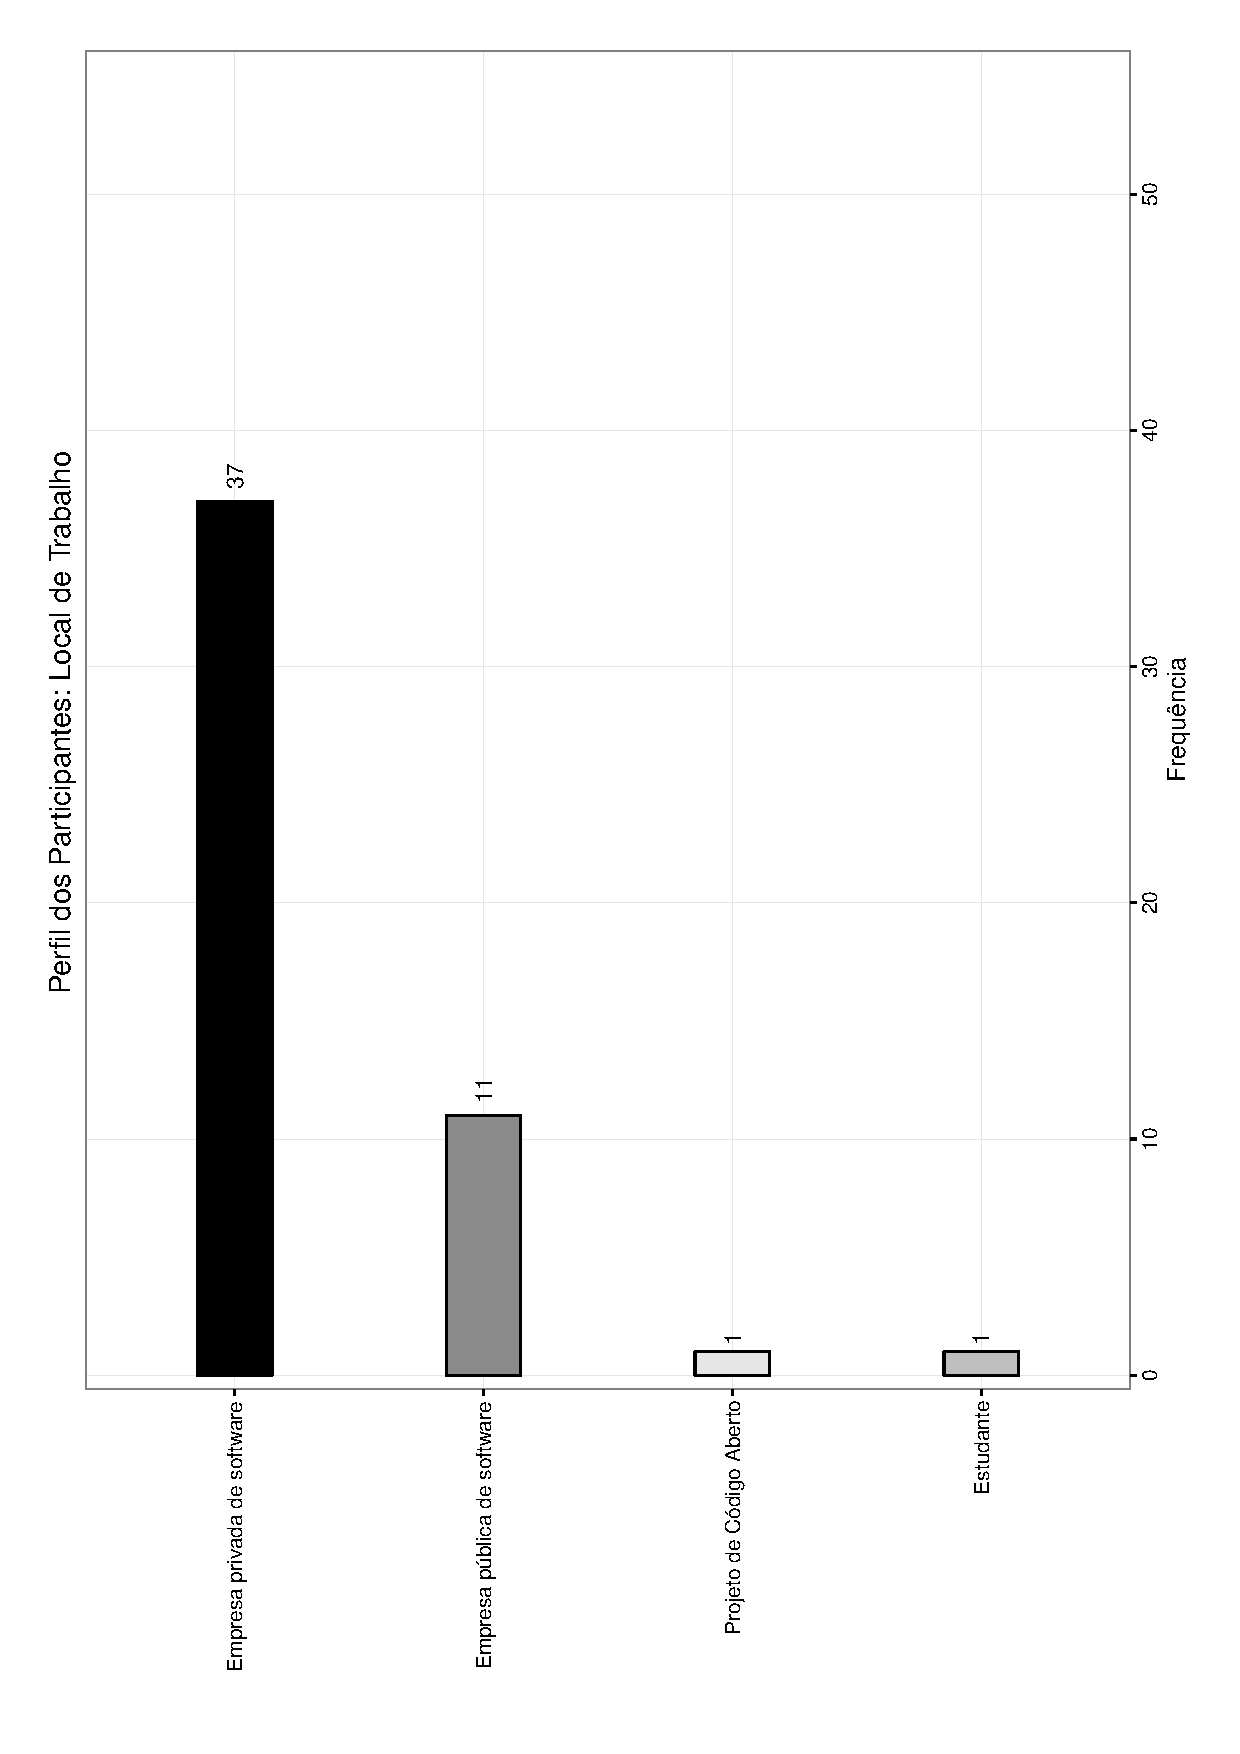
\includegraphics[width=0.8\linewidth]{./chapter-estudo-funcionalidades-fgrm/img/grafico_escolha_ferramentas_local_trabalho.pdf}
	\caption{Local de trabalho}
	\label{fig:grafico_escolha_ferramentas_local_trabalho}
\end{figure}

\subsection{Ferramentas Escolhidas}
\label{subsec:resultados_ferramentas_escolhidas}

Utilizando a Equação~\ref{eq:escolha_ferramenta} obtivemos as ferramentas
apresentas na Tabela~\ref{tab:ferramenta_utilizadas_estudo}. Conforme pode ser
observado foi escolhido três softwares de cada tipo (ferramenta e serviço da
Internet). É importante perceber que as FGRMs \textit{Github e Gitlab} não
estavam na lista inicial, contudo, apareceram neste resultado final. Isso
decorre  de atribuímos o maior peso ($w_i = 5$) para aquelas ferramentas que
foram citadas pelos participantes de maneira espontânea.  Neste caso, devido a
frequência que estas ferramentas elas acabaram escolhidas.

\begin{table}[htb]
\centering
\caption{Ferramentas utilizados no estudo}
\label{tab:ferramenta_utilizadas_estudo}
\resizebox{\textwidth}{!}{%
\begin{tabular}{|lccl|}
\hline
\multicolumn{1}{|c}{\textbf{Ferramenta}} & \textbf{Classificação} & \textbf{Versão} & \multicolumn{1}{c|}{\textbf{URL}}      \\ \hline
Bugzilla                                 & Ferramenta             & 5.0.3           & https://www.bugzilla.org               \\
Mantis Bug Tracker                       & Ferramenta             & 1.3.2           & https://www.mantisbt.org               \\
Redmine                                  & Ferramenta             & 3.3.1           & http://www.redmine.org/                \\
JIRA Software                            & Serviço                & 7.2.4           & https://br.atlassian.com/software/jira \\
Github Issue System             & Serviço                & \@-\@           & https://github.com/                    \\
Gitlab Issue Tracking System             & Serviço                & \@-\@           & https://gitlab.com/                    \\ \hline
\end{tabular}%
}
\end{table}


\subsection{Espectro de Funcionalidades das FGRMs}
\label{subsec:categorizacao_ferramentas}

\todobegin{Incluída uma classificação das funcionalidades nas dimensões Gestão da
RM, Ferramenta e Processo}

Após a inspeção da documentação e validação dos dados obtivemos um total de 123
cartões. Nós sistematizamos os cartões manualmente tendo em vista que não
existem ferramentas ou métodos capazes de automatizar o processo de construção
de hi\-e\-rar\-qui-\-as. Como o nosso objetivo é derivar tópicos a partir de um
conjunto inicial de cartões, optamos por realizar um \textit{ordenamento
	aberto}. Neste tipo de abordagem, os grupos são estabelecidos durante o
processo de classificação dos cartões em oposição a outra forma de utilização da
técnica onde a sistematização dos cartões ocorre com base em grupos
pré-determinados. Ao final do processo compilamos os tópicos de modo a construir
um espectro de funcionalidades para as FGRM que pode observado na
Figura~\ref{fig:diagrama-espectro-funcionalidades-fgrm}, no qual temos três
dimensões de funcionalidades que são compostas por diferentes categorias de
funcionalidades.

\begin{figure}[htpb]
	\centering
	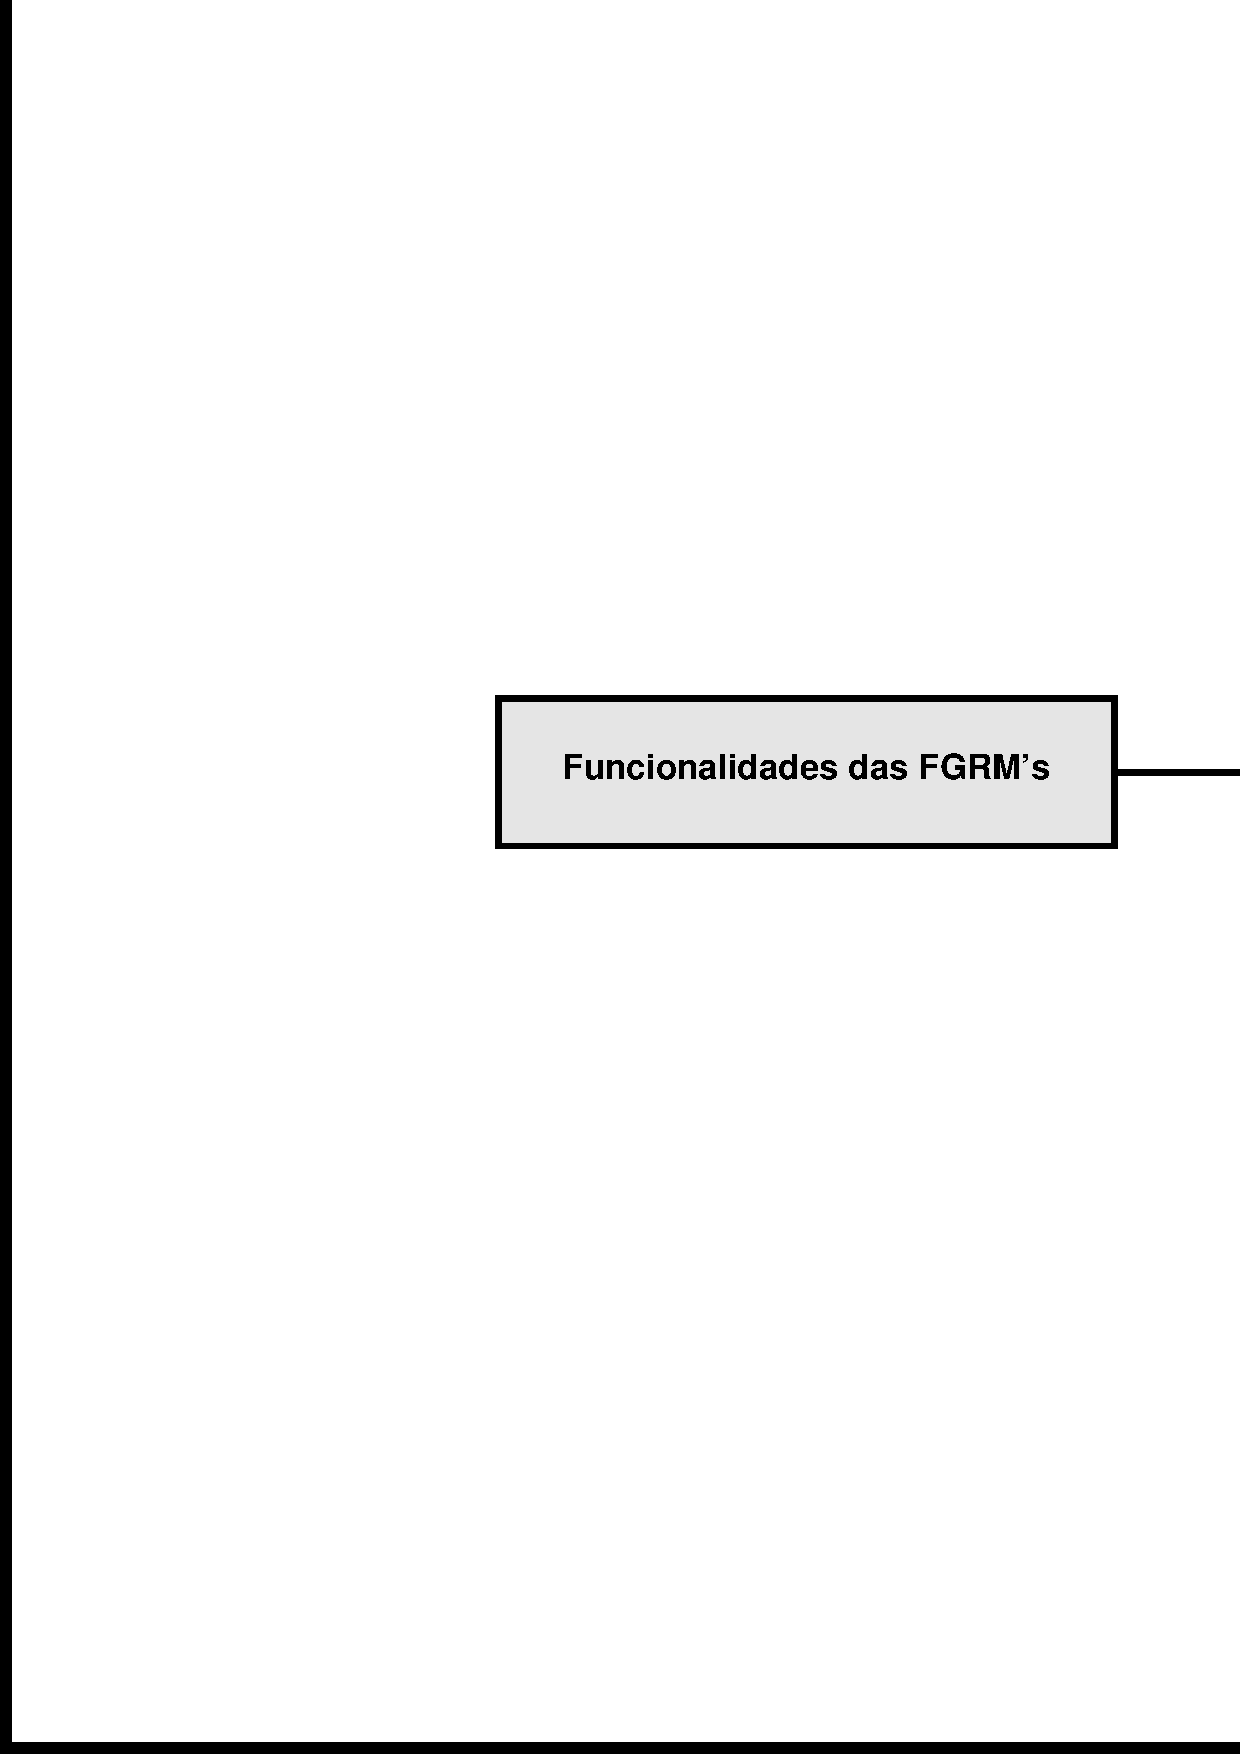
\includegraphics[width=1.15\linewidth]{./chapter-estudo-funcionalidades-fgrm/img/diagrama-espectro-funcionalidades-fgrm.pdf}
	\caption{Dimensões técnicas de uma FGRM}
	\label{fig:diagrama-espectro-funcionalidades-fgrm}
\end{figure}

A figura foi construída com base nas categorias de funcionalidades exibidas na
Tabela~\ref{tab:freq_categorias_cartoes} onde é possível verificar ainda a
frequência que cada uma das categorias apareceu no conjunto de cartões
coletado.

\begin{table}[htpb]
\centering
\resizebox{.7\textwidth}{!}{%
\begin{tabular}{|l|c|}
\hline
\multicolumn{1}{|c|}{\textbf{Categoria de Funcionalidades}} & \textbf{Frequência} \\ \hline
Operações de CRUD & 24 \\
Visualização e Monitoramento de RMs & 22 \\
Segurança da Informação & 17 \\
Fluxo de Trabalho & 15 \\
Interfaces de Notificação & 13 \\
Extensão de Funcionalidades & 8 \\
Triagem de RMs & 6 \\
Gerenciamento de Artefatos & 6 \\
Integração com Sistemas de Controle de Versão & 4 \\
Gerenciamento da Informação & 4 \\
Internacionalização da Ferramenta & 3 \\
Auditoria & 1 \\ \hline
\end{tabular}%
}
\caption{Frequência de cada categoria de funcionalidade no conjunto de cartões
	obtidos.}
\label{tab:freq_categorias_cartoes}
\end{table}

\subsubsection{Gestão da RM}
\label{ssub:gestao_da_rm}

O gerenciamento da RMs formam as funcionalidades centrais de uma FGRM. De uma
maneira geral, uma das primeira responsabilidades de uma FGRM é gerir a
\textit{criação, consulta, atualização e destruição} de uma RM. Estas funções
podem ser agrupadas em um termo único denominado \textit{Operações de CRUD}
(acrônimo de Create, Read, Update e Delete na língua Inglesa). As principais
categorias de funcionalidades que foram encontradas para a dimensão de
\textit{Gestão da RM} estão descritas a seguir.

\paragraph{Operações de CRUD:}
\label{par:operações_de_crud}

Nesta categoria estão as funcionalidades que dão suporte à criação,	consulta,
atualização e destruição das RMs. Com relação à criação verificamos que algumas
FGRM possibilitam a definição de \textit{campos customizáveis} para o
preenchimento da RM. A ferramenta Bugzilla suporta a adição de campos
personalizados ao seu banco de dados de RMs de modo à capturar e pesquisar
dados que são exclusivo do projeto ao qual dará suporte. Estes campos podem
ainda ser exibidos com base no valor de um outro, para usá-los apenas quando for
relevante.

Esta categoria também agrupa as funcionalidades relacionadas a busca de RMs e a
localização de duplicados. Durante o processo de criação de uma RM, uma das
ferramentas possui a funcionalidade  para detecção automatizada de duplicados.
Para criar uma nova RMs algumas ferramentas possibilitam diferentes
\textit{interfaces de entrada} de modo que uma RM pode ser criada através do
envio de e-mail, utilizando dispositivos móveis ou mediante formulários próprios
criados em qualquer site da web.

Verificamos ainda que algumas FGRM permitem que o relato da RM seja realizado em
linguagem de marcação como o
Markdown\footnote{\url{https://en.wikipedia.org/wiki/Markdown}}, que permite
entre outras coisas a inclusão de código fonte com a sintaxe realçada. Isso
possibilita visualizar de forma mais clara partes do código fonte podem ser
incluídas na RM. Neste mesmo tópico encontramos funcionalidades para recuperar
uma RM utilizando o texto relato em uma RM, mediante filtros personalizáveis ou
por meio de uma Linguagem de Domínio Específico (Domain-Specific Language - DSL
em inglês) baseada em SQL.

\paragraph{Gerenciamento da Informação}
\label{par:gerenciamento_da_informação}

Dentro de um projeto de desenvolvimento ou manutenção de software gerenciar uma
RM por vez não é muito eficiente. Neste sentido, é necessário que as FGRMs
suportem RMs de forma agregada permitindo o gerenciamento em massa da
informação armazenada. Este tópico contempla as funcionalidades que se dedicam
ao armazenamento e consistência das informações contidas na FGRM. As ferramentas
possuem funcionalidades para \textit{suportar múltiplas bases de dados}, como os
diferentes Sistemas de Gerenciamento de Banco de Dados disponíveis no mercado.
Além disso, a ferramenta Bugzilla oferece funcionalidade própria para validação
de consistências dos dados armazenados.

\subsubsection{Ferramenta}
\label{ssub:ferramenta}

As FGRM devem fornecer recursos através dos quais outras ferramentas possam
interagir e manipular a informação que elas armazenam. Nesta dimensão estão as
funcionalidades que permitem manipulação externa dos dados contidos nas RMs ou
mesmo o desenvolvimento de novas funções ou comportamentos da FGRM mediante o
uso de APIs
\footnote{\url{https://en.wikipedia.org/wiki/Application_programming_interface}}
e extensões.

\paragraph{Extensão de Funcionalidades}
\label{par:extensão_de_funcionalidades}

As funcionalidades que compõem este grupo têm por objetivo entender o conjunto
de funcionalidades oferecidas através de uma arquitetura de plugins ou mediante
o suporte de APIs. Algumas ferramentas como o Github permitem realizar as
atividades de gestão de uma RM mediante a utilização de uma API própria. No caso
do Bugzilla e do Mantis é permitido o acesso à informação das RMs através de
Webservice.

\paragraph{Integração com Sistemas de Controle de Versão}
\label{par:integração_com_sistemas_de_controle_de_versão}

As FGRM podem acessar os repositórios de código de fonte, gerenciados mediante
um Sistema de Controle de Versão (SCV), permitindo que o usuário navegue pelo
seu conteúdo, visualize e procure o conjunto de alterações realizadas. As
ferramentas também possibilitam acesso à diferentes tipos de SCV, tais como Git,
SVN, Mercurial e etc.

\paragraph{Interfaces de Notificação}
\label{par:interfaces_de_notificação}

Neste tópico estão as funcionalidades oferecidas pelas FGRMs para notificar as
diversas partes interessadas envolvidas em determinado projeto de software. As
FGRMs podem notificar através de e-mail, RSS, Twitter e chats.

\subsubsection{Processo}
\label{ssub:processo}

Esta dimensão foi criada para agrupar as funcionalidades que dão suporte ao
processo de manter software, demostrando que as FGRM gerenciam, além da própria
RM, as pessoas e artefatos que colaboram no desenvolvimento e manutenção de
software.

\paragraph{Fluxo de trabalho}
\label{par:fluxo_de_trabalho}

Nesta categoria que dão suporte ao processo de trabalho adotado no
desenvolvimento e manutenção de software. Nele estão incluídos funcionalidade
para gerenciamento de tarefas e suporte à múltiplos projetos. Também é possível
personalizar o fluxo de trabalho adotado. Esta customização é realizada através
da definição de \textit{situações} próprias que se adéquem às necessidades do
projeto.

\paragraph{Gerenciamento de Artefatos}
\label{par:gerenciamento_de_artefatos}

O processo de manutenção de software pode consumir ou gerar diversos artefatos,
tais como documentos de requisitos e arquiteturais dos software, código fonte,
registros (logs) de teste e assim por diante~\cite{cavalcanti2013bug}. Em alguns
contextos, devido ao volume de artefato gerados, é importante que a FGRM dê
suporte para armazenamento e recuperação deste ativos do processo de software.
As FGRMs possuem funcionalidades que interagem diretamente com a documentação
de software, geralmente no formato de Wiki. Além disso algumas ferramentas
permitem uma melhor visualização de anexos incluídos na RM, especialmente
aqueles em formato texto como arquivos CSV.

\paragraph{Triagem de RMs}
\label{par:triagem_de_rm_s}

Este tópico descreve as funcionalidades relacionadas com o processo de triagem
de RMs. O processo de atribuição de RM, também conhecido como triagem, possui
como principal objetivo encontrar o desenvolvedor mais capacitado para manipular
uma dada RM\@. As FGRMs dão suporte a esta atividade principalmente através da
categorização das RMs. Todas as ferramentas analisadas permitem algum tipo de
classificação através do uso de etiquetas.

\paragraph{Internacionalização da Ferramenta}
\label{par:internacionalização_da_ferramenta}

Neste tópicos estão as características das FGRM que ajudam no desenvolvimento
e/ou adaptação de um produto, em geral softwares de computadores, para uma
língua e cultura de um país. As FGRM possuem tradução para diversos idiomas e
também possuem funcionalidades que permitem à colaboradores criarem novas
traduções.

\paragraph{Segurança da Informação}
\label{par:segurança_da_informação}

Neste grupo estão as funcionalidades de uma FGRM que diretamente relacionada com
proteção de um conjunto de informações, no sentido de preservar o valor que
possuem para um indivíduo ou uma organização. Assim as ferramentas oferecem
funcionalidades para suporte à confidencialidade, integridade e autenticidade da
informação armazenada.

\paragraph{Visualização e Monitoramento de RMs}
\label{par:visualização_de_rm_s}

Em diversos contextos, devido ao volume das RMs, é importante que as partes
interessadas na manutenção de software, possam visualizar e monitorar a situação
das requisições que estão analisadas em determinado período. Neste contexto, as
FGRM oferecem funcionalidades para visualizar a informação das RMs mediante
quadro como aqueles utilizados nas metodologias Kanban ou SCRUM. Existem
funcionalidades que permitem ao usuário visualizar um conjunto específico de
RMs. Neste mesma categoria estão as funcionalidades para geração de relatório
que ajudam aos gerentes do projeto na tomada de decisão.

\section{Discussão}
\label{sec:discussao}

Para algumas funcionalidades não há uma separação clara em qual categoria ela
pode ser encaixada, como por exemplo a possibilidade que algumas FGRM fornecem
de personalizar os campos que compõem uma RM. Esta função está relacionada com a
criação da RM (Operação de CRUD), contudo, também faz parte da definição de
processo de trabalho próprio de um projeto, o que poderia categorizá-la como
Fluxo de Trabalho. Esta mesma situação ocorre com as funcionalidades de deleção
de uma RM que foram classificadas como \textit{Operações de CRUD}, mas que tem
relação com a categoria de \textit{Segurança da Informação} já que para realizar
tal ação o usuário deve ser identificado (login realizado no sistema) e
autorizado para tal.

A análise das funcionalidades nos permite verificar que as tarefas das FGRM
evoluíram de simplesmente gerenciar as RM para colaborar no processo de
desenvolvimento e manutenção de software. Todavia, esta evolução não é tão
rápida quanto o necessário. As ferramentas apresentam um suporte bem
estabelecido para atividades relativas à gestão da RM, como por exemplo a
criação de uma nova RM. Contudo, ainda é bastante escasso funcionalidades que
minimizem os problemas que ocorrem quando as RMs são geradas, como por exemplo,
duplicadas ou baixa qualidade do relato.

É possível verificar que as FGRM oferecem funcionalidades que dão suporte a todo
o ciclo de vida de uma RM, conforme discutido na
Subseção~\ref{sub:fluxo_de_trabalho_requisicao_mudanca}. Todavia, grande parte
do esforço fica a cargo do usuário da ferramenta, o que pode resultar em atrasos
em situações em que se tem muitas RM para gerenciar. Um exemplo deste problema
ocorre no processo de atribuição do Desenvolvedor responsável por solucionar
determinada RM. Conforme discutido no Capítulo~\ref{ch:visao-geral-manutencao}
esta atividade fica sob a responsabilidade do \textit{Agendador}. Ele deve
realizar a escolha de forma manual tendo em vistas que as FGRM não apresentam
funcionalidades que sejam capaz de ` `recomendar'' o desenvolvedor mais apto.

As FGRMs possuem funcionalidades que permitem a realização do papel ao qual
este tipo de software se propõe. Não obstante, devido à sua crescente
importância, é importante que este tipo de ferramenta incorpore funções e
comportamentos que ajudem no processo de desenvolvimento e manutenção de
software, especialmente em áreas como busca de duplicados, melhoria do relato e
atribuição e classificação automatizadas.

\section{Ameaças à Validade}
\label{sec:ameacas_a_validade}

Classificar envolve categorização, e há uma literatura sofisticada sobre
categorização, taxonomia e semântica, todas as quais são potencialmente
relevantes~\cite{rugg2005sorting}. Em grande parte dos estudos a generalidade
dos resultados é muitas vezes sacrificada pela riqueza e complexidade dos dados
analisados. Neste sentido, podemos afirmar que o processo de classificação é,
por natureza, uma avaliação subjetiva.

Uma ameaça à validade do trabalho está no processo de seleção das ferramentas.
Apesar da escolha ter sido realizada com suporte de profissionais envolvido em
manutenção de software, não podemos garantir que o número de respondentes pode
suportar que foi escolhido as ferramentas mais relevantes dentre aquelas
disponíveis. Neste mesmo sentido, a formula que foi utilizada para definir as
mais relevantes podem conter um enviesamentos sobretudo pela forma que os pesos
foram adotados, ou seja, não há como garantir que o fato de um participante
entender que uma determinada ferramenta é muito relevante ($w_j = 5$) mereça ser
ponderado cinco vezes mais que uma outra que não é conhecida ($w_j = 1$).
Todavia ao bem do nosso conhecimento não há técnicas para classificação que não
tenha influência da subjetividade.

Com relação à técnica de classificação utilizando Cartões de Ordenamento temos
dois pontos principais de ameaças aos resultados. Como a extração dos dados foi
realizada de forma manual pode ter ocorrido algum tipo de equívoco no processo
como por exemplo a  não coleta de determinada ferramenta por mero esquecimento.
Todavia, um número pequeno de ferramentas foi selecionada tendo em vista a
limitação desta extração manual. Um segundo ponto encontra-se na classificação
dos cartões. Apesar do processo ter sido realizado em pares pode ter ocorrido
uma classificação de forma incorreta o que pode acarretar em limitação dos
resultados apresentados. Esta situação pode ocorrer porque para algumas
funcionalidades não há uma fronteira clara para qual grupo ela pertence.

\section{Resumo do Capítulo}
\label{sec:resumo_do_capitulo}
\todobegin{Aguardando a revisão final do capítulo para realizar a escrita desta
seção.}
